% Options for packages loaded elsewhere
\PassOptionsToPackage{unicode}{hyperref}
\PassOptionsToPackage{hyphens}{url}
%
\documentclass[
]{article}
\usepackage{amsmath,amssymb}
\usepackage{iftex}
\ifPDFTeX
  \usepackage[T1]{fontenc}
  \usepackage[utf8]{inputenc}
  \usepackage{textcomp} % provide euro and other symbols
\else % if luatex or xetex
  \usepackage{unicode-math} % this also loads fontspec
  \defaultfontfeatures{Scale=MatchLowercase}
  \defaultfontfeatures[\rmfamily]{Ligatures=TeX,Scale=1}
\fi
\usepackage{lmodern}
\ifPDFTeX\else
  % xetex/luatex font selection
  \setmainfont[]{TeX Gyre Pagella}
\fi
% Use upquote if available, for straight quotes in verbatim environments
\IfFileExists{upquote.sty}{\usepackage{upquote}}{}
\IfFileExists{microtype.sty}{% use microtype if available
  \usepackage[]{microtype}
  \UseMicrotypeSet[protrusion]{basicmath} % disable protrusion for tt fonts
}{}
\makeatletter
\@ifundefined{KOMAClassName}{% if non-KOMA class
  \IfFileExists{parskip.sty}{%
    \usepackage{parskip}
  }{% else
    \setlength{\parindent}{0pt}
    \setlength{\parskip}{6pt plus 2pt minus 1pt}}
}{% if KOMA class
  \KOMAoptions{parskip=half}}
\makeatother
\usepackage{xcolor}
\usepackage[margin=1in]{geometry}
\usepackage{longtable,booktabs,array}
\usepackage{calc} % for calculating minipage widths
% Correct order of tables after \paragraph or \subparagraph
\usepackage{etoolbox}
\makeatletter
\patchcmd\longtable{\par}{\if@noskipsec\mbox{}\fi\par}{}{}
\makeatother
% Allow footnotes in longtable head/foot
\IfFileExists{footnotehyper.sty}{\usepackage{footnotehyper}}{\usepackage{footnote}}
\makesavenoteenv{longtable}
\usepackage{graphicx}
\makeatletter
\def\maxwidth{\ifdim\Gin@nat@width>\linewidth\linewidth\else\Gin@nat@width\fi}
\def\maxheight{\ifdim\Gin@nat@height>\textheight\textheight\else\Gin@nat@height\fi}
\makeatother
% Scale images if necessary, so that they will not overflow the page
% margins by default, and it is still possible to overwrite the defaults
% using explicit options in \includegraphics[width, height, ...]{}
\setkeys{Gin}{width=\maxwidth,height=\maxheight,keepaspectratio}
% Set default figure placement to htbp
\makeatletter
\def\fps@figure{htbp}
\makeatother
\setlength{\emergencystretch}{3em} % prevent overfull lines
\providecommand{\tightlist}{%
  \setlength{\itemsep}{0pt}\setlength{\parskip}{0pt}}
\setcounter{secnumdepth}{5}
\let\oldthefigure\thefigure
\renewcommand{\thefigure}{S\oldthefigure}
\let\oldthetable\thetable
\renewcommand{\thetable}{S\oldthetable}
\usepackage{booktabs}
\usepackage{longtable}
\usepackage{array}
\usepackage{multirow}
\usepackage{wrapfig}
\usepackage{float}
\usepackage{colortbl}
\usepackage{pdflscape}
\usepackage{tabu}
\usepackage{threeparttable}
\usepackage{threeparttablex}
\usepackage[normalem]{ulem}
\usepackage{makecell}
\usepackage{xcolor}
\ifLuaTeX
  \usepackage{selnolig}  % disable illegal ligatures
\fi
\IfFileExists{bookmark.sty}{\usepackage{bookmark}}{\usepackage{hyperref}}
\IfFileExists{xurl.sty}{\usepackage{xurl}}{} % add URL line breaks if available
\urlstyle{same}
\hypersetup{
  pdftitle={COATi: statistical pairwise alignment of protein coding sequences},
  pdfauthor={Juan J. Garcia Mesa, Ziqi Zhu, Reed A. Cartwright},
  hidelinks,
  pdfcreator={LaTeX via pandoc}}

\title{COATi: statistical pairwise alignment of protein coding sequences}
\usepackage{etoolbox}
\makeatletter
\providecommand{\subtitle}[1]{% add subtitle to \maketitle
  \apptocmd{\@title}{\par {\large #1 \par}}{}{}
}
\makeatother
\subtitle{Supplementary Materials}
\author{Juan J. Garcia Mesa, Ziqi Zhu, Reed A. Cartwright}
\date{}

\begin{document}
\maketitle

{
\setcounter{tocdepth}{2}
\tableofcontents
}
\section{Aligner Commands}\label{aligner-commands}

We evaluated five different aligners. Below are the commands that we used to run
them. We have abbreviated the commands for clarity, stripping out unimportant
arguments. Complete workflows can be found in our coati-testing repository on
Github.

\begin{itemize}
\tightlist
\item
  COATi: \texttt{coati\ alignpair\ -m\ tri-mg\ ...}; We used COATi two different ways. The
  primary way used human as the reference sequence. The secondary way,
  COATi-rev, used gorilla as the reference, via a wrapper script that reversed
  the order of sequences before alignment and reversed the order back
  afterwards.
\item
  ClustalΩ v1.2.4: \texttt{clustalo\ -\/-seqtype=Protein\ ...}; We wrapped ClustalΩ with a
  script that translates DNA sequences into amino acid sequences (including
  stops) before alignment. Any codons that were partial or containing ambiguous
  characters were translated as ``X''. The script then aligned these translated
  sequences with ClustalΩ, and then created a DNA alignment that was consistent
  with the amino-acid alignment.
\item
  MACSE v2.06: \texttt{java\ -jar\ macse.jar\ -prog\ alignSequences\ -seq\ human.fasta\ \ \ -seq\_lr\ gorilla.fasta\ ...}; We wrapped MACSE with a script that created two
  temporary fasta files, one containing the human sequence and another
  containing the gorilla sequence. The human sequence was specified as the
  reliable sequence and the gorilla sequence was specified as the less-reliable
  sequence. MACSE uses ``!'' to mark gaps that result from frameshifts, and the
  wrapper script replaced these with ``-''. Additionally, MACSE sometimes produced
  columns that only contained gaps, and these columns were removed.
\item
  PRANK v.150803: \texttt{prank\ -codon\ ...}
\item
  MAFFT v7.520: \texttt{mafft\ -\/-preservecase\ -\/-globalpair\ -\/-maxiterate\ 1000\ ...}
\end{itemize}

COATi can use different alignment models for pairwise alignment. Below are the
commands that we used to run different models.

\begin{itemize}
\tightlist
\item
  tri-mg: \texttt{coati\ alignpair\ -m\ tri-mg\ ...}
\item
  tri-ecm: \texttt{coati\ alignpair\ -m\ tri-ecm\ ...}
\item
  mar-mg: \texttt{coati\ alignpair\ -m\ mar-mg\ ...}
\item
  mar-ecm: \texttt{coati\ alignpair\ -m\ mar-ecm\ ...}
\end{itemize}

\section{FST Alignment Example}\label{fst-alignment-example}

When using the triplet models (tri-mg and tri-ecm), COATi uses the OpenFST
library to generate best alignments by composing the input and output sequences
with the COATi FST model. While the COATi FST model is too large to display, we
can show the result of a composition.

Fig. \ref{fig:aln-example-a} shows a graph depicting the FST that results from
composing the COATi FST with the input sequence ``CTC'' and the output sequence
``CTG''. Every path through this FST represents one possible way to align ``CTC''
and ``CTG'', and the sum of all weights along a path is the total weight of the
respective alignment. Here, the weights of each arc are in negative-log space.
Note that this graph has been optimized, and weight has been pushed towards the
initial state. The weight of any specific arc may not be directly mapable to a
weight described in the model.

Fig. \ref{fig:aln-example-b} is the best alignment between ``CTC'' and ``CTG'', as
determined by the shortest path algorithm. Figs. \ref{fig:aln-example-a} and
\ref{fig:aln-example-b} were produced by the OpenFST library. A bold circle
represents a starting node, and a double circle represents a termination node.

\begin{figure}

{\centering 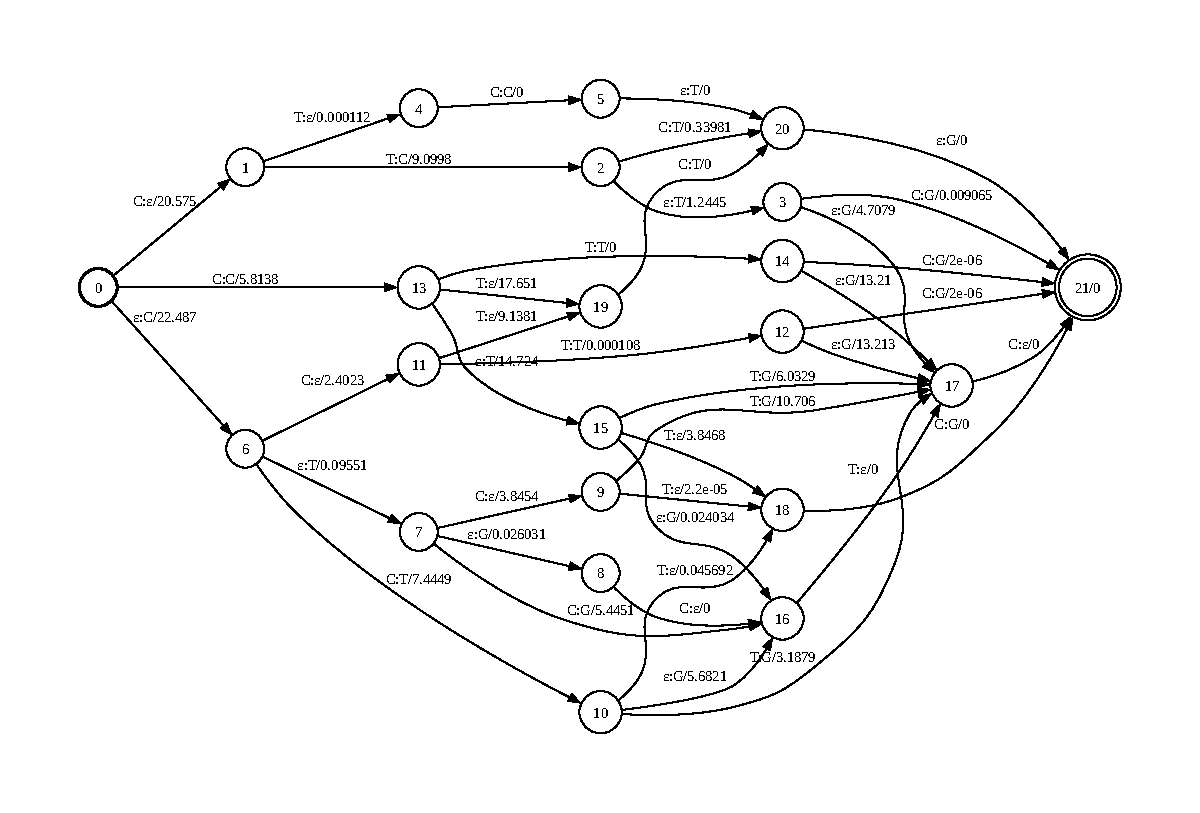
\includegraphics{figures/aln-example-graph} 

}

\caption{The FST of all possible alignments between "CTC" and "CTG".}\label{fig:aln-example-a}
\end{figure}

\begin{figure}

{\centering 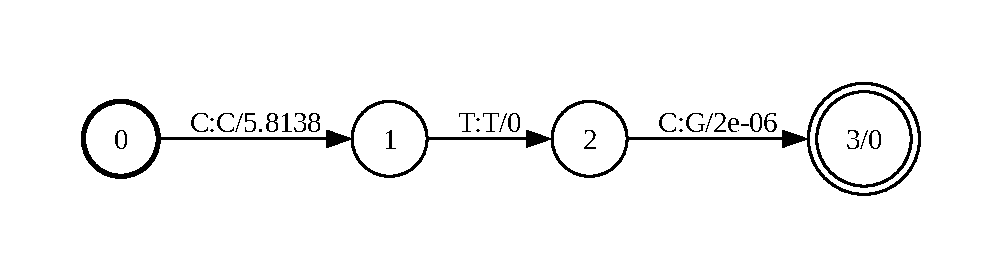
\includegraphics[width=0.75\linewidth]{figures/aln-example-path} 

}

\caption{The best alignment of "CTC" and "CTG".}\label{fig:aln-example-b}
\end{figure}

\newpage

\section{Empirical Results}\label{empirical-results}

\subsection{Gap Patterns}\label{gap-patterns}

\subsubsection{Lengths}\label{lengths}

We quantified the lengths of gaps produced by each method across the empirical
dataset of human-gorilla protein-coding-sequence pairs (Tab. @ref
(tab:gap-table-1)). Here the gap type is either ``D'' for gaps introduced into
the gorilla sequence or ``I'' for gaps introduced in the human sequence. ``COATi''
refers to the full COATi FST model with a MG substitution model
(i.e.~tri-mg). ``COATi-rev'' refers to the same model, but using gorilla as the
reference and human as the non-reference sequence. Gap lengths of 1--6
nucleotides were binned into their respective columns. Gap lengths longer than
6 nucleotides were binned into columns 7+, 8+, and 9+ depending on whether
their lengths were 1, 2, or 3 nucleotides longer than a multiple of three.

We also quantified the lengths of gaps produced by different COATi models
(Tab. \ref{tab:gap-table-2}).

Note that ClustalΩ gaps with lengths that are not a multiple of 3 are created by
how our wrapper script handles DNA sequences with lengths that are not multiple
of 3.

\begin{table}[H]
\centering
\caption{\label{tab:gap-table-1}Number of gaps introduced by each method separated by length and type.}
\centering
\begin{tabular}[t]{lcrrrrrrrrr}
\toprule
\multicolumn{2}{c}{ } & \multicolumn{9}{c}{Gap Lengths} \\
\cmidrule(l{3pt}r{3pt}){3-11}
Method & Gap Type & 1 & 2 & 3 & 4 & 5 & 6 & 7+ & 8+ & 9+\\
\midrule
COATi & D & 106 & 99 & 651 & 94 & 94 & 226 & 1461 & 1386 & 3240\\
COATi & I & 87 & 73 & 525 & 80 & 97 & 239 & 1399 & 1315 & 3105\\
\addlinespace
COATi-rev & D & 105 & 99 & 634 & 89 & 96 & 217 & 1425 & 1348 & 3169\\
COATi-rev & I & 82 & 79 & 513 & 80 & 97 & 231 & 1360 & 1288 & 3031\\
\addlinespace
ClustalΩ & D & 1 & 0 & 887 & 1 & 1 & 400 & 3 & 7 & 3910\\
ClustalΩ & I & 0 & 0 & 857 & 0 & 1 & 424 & 3 & 2 & 3747\\
\addlinespace
MACSE & D & 396 & 306 & 1237 & 5 & 3 & 657 & 71 & 54 & 4784\\
MACSE & I & 60 & 27 & 1133 & 5 & 9 & 666 & 78 & 97 & 4381\\
\addlinespace
MAFFT & D & 204 & 156 & 714 & 147 & 108 & 276 & 544 & 509 & 2680\\
MAFFT & I & 187 & 154 & 708 & 112 & 92 & 295 & 454 & 424 & 2642\\
\addlinespace
PRANK & D & 0 & 0 & 552 & 0 & 0 & 167 & 0 & 0 & 4812\\
PRANK & I & 0 & 0 & 467 & 0 & 0 & 178 & 0 & 0 & 4686\\
\bottomrule
\end{tabular}
\end{table}

\begin{table}[H]
\centering
\caption{\label{tab:gap-table-2}Number of gaps introduced by different COATi models separated by length and type.}
\centering
\begin{tabular}[t]{lcrrrrrrrrr}
\toprule
\multicolumn{2}{c}{ } & \multicolumn{9}{c}{Gap Lengths} \\
\cmidrule(l{3pt}r{3pt}){3-11}
Model & Gap Type & 1 & 2 & 3 & 4 & 5 & 6 & 7+ & 8+ & 9+\\
\midrule
TRI-MG & D & 106 & 99 & 651 & 94 & 94 & 226 & 1461 & 1386 & 3240\\
TRI-MG & I & 87 & 73 & 525 & 80 & 97 & 239 & 1399 & 1315 & 3105\\
\addlinespace
TRI-ECM & D & 93 & 96 & 665 & 125 & 122 & 257 & 1438 & 1441 & 3203\\
TRI-ECM & I & 86 & 103 & 540 & 105 & 122 & 254 & 1358 & 1370 & 3099\\
\addlinespace
MAR-MG & D & 102 & 106 & 646 & 95 & 89 & 224 & 1465 & 1399 & 3226\\
MAR-MG & I & 84 & 83 & 526 & 80 & 101 & 238 & 1406 & 1313 & 3087\\
\addlinespace
MAR-ECM & D & 110 & 110 & 653 & 107 & 89 & 224 & 1424 & 1389 & 3250\\
MAR-ECM & I & 86 & 89 & 523 & 77 & 99 & 249 & 1408 & 1310 & 3128\\
\addlinespace
DNA & D & 101 & 103 & 646 & 95 & 91 & 224 & 1446 & 1409 & 3206\\
DNA & I & 79 & 79 & 520 & 78 & 99 & 239 & 1369 & 1316 & 3107\\
\bottomrule
\end{tabular}
\end{table}

\subsubsection{Phases}\label{phases}

We quantified the phases of gaps produced by different aligners and COATi
models (Tab. \ref{tab:gap-table-3} and \ref{tab:gap-table-4}). Phase 1 gaps
begin after the 1st position in a codon in the reference sequence, phase 2 gaps
begin after the 2nd position in a codon, and phase 3 begin after the 3rd
position in a codon (i.e.~between codons). Phase 3 gaps are also known as phase
0 gaps.

Note that ClustalΩ gaps with phases of 1 and 2 are created by how our wrapper
script handles DNA sequences with lengths that are not multiple of 3.

\begin{table}[H]
\centering
\caption{\label{tab:gap-table-3}Number of gaps introduced by each alignment method separated by phase.}
\centering
\begin{tabular}[t]{lrrr}
\toprule
\multicolumn{1}{c}{ } & \multicolumn{3}{c}{Gap Phases} \\
\cmidrule(l{3pt}r{3pt}){2-4}
Method & 1 & 2 & 3\\
\midrule
COATi & 4493 & 3962 & 5822\\
\addlinespace
COATi-rev & 3992 & 3775 & 6176\\
\addlinespace
ClustalΩ & 8 & 6 & 10230\\
\addlinespace
MACSE & 455 & 497 & 13017\\
\addlinespace
MAFFT & 2317 & 2631 & 5458\\
\addlinespace
PRANK & 0 & 0 & 10862\\
\bottomrule
\end{tabular}
\end{table}

\begin{table}[H]
\centering
\caption{\label{tab:gap-table-4}Number of gaps introduced by different COATi models separated by phase.}
\centering
\begin{tabular}[t]{lrrr}
\toprule
\multicolumn{1}{c}{ } & \multicolumn{3}{c}{Gap Phases} \\
\cmidrule(l{3pt}r{3pt}){2-4}
Model & 1 & 2 & 3\\
\midrule
TRI-MG & 4493 & 3962 & 5822\\
\addlinespace
TRI-ECM & 4160 & 4678 & 5639\\
\addlinespace
MAR-MG & 4130 & 3961 & 6179\\
\addlinespace
MAR-ECM & 4071 & 3863 & 6391\\
\addlinespace
DNA & 4228 & 3974 & 6005\\
\bottomrule
\end{tabular}
\end{table}

\subsection{Homology Patterns}\label{homology-patterns}

We quantified the homology patterns of residues for different aligners and COATi
models (Tab. \ref{tab:gap-table-5}, Tab. \ref{tab:gap-table-6}, and
Fig. \ref{fig:gap-figure-1}). Here we define the match, mismatch, and gap
percentages as the percent of nucleotides aligned against a match, mismatch,
and gap respectively. Note that this is different than the percent of columns
that contain a match, mismatch, or gap because match and mismatch columns are
counted twice.

\begin{table}[H]
\centering
\caption{\label{tab:gap-table-5}Average homology percentages of alignments separated by alignment method.}
\centering
\begin{tabular}[t]{rccc}
\toprule
Method & Matches & Mismatches & Gaps\\
\midrule
COATi & 95.93\% & 0.79\% & 3.28\%\\
\addlinespace
COATi-rev & 95.95\% & 0.79\% & 3.25\%\\
\addlinespace
ClustalΩ & 95.93\% & 1.54\% & 2.52\%\\
\addlinespace
MACSE & 96.13\% & 1.33\% & 2.54\%\\
\addlinespace
MAFFT & 96.12\% & 1.36\% & 2.52\%\\
\addlinespace
PRANK & 95.64\% & 0.84\% & 3.52\%\\
\bottomrule
\end{tabular}
\end{table}

\begin{table}[H]
\centering
\caption{\label{tab:gap-table-6}Average homology percentages of alignments separated by COATi model.}
\centering
\begin{tabular}[t]{rccc}
\toprule
Model & Matches & Mismatches & Gaps\\
\midrule
TRI-MG & 95.93\% & 0.79\% & 3.28\%\\
\addlinespace
TRI-ECM & 95.90\% & 0.79\% & 3.30\%\\
\addlinespace
MAR-MG & 95.93\% & 0.79\% & 3.28\%\\
\addlinespace
MAR-ECM & 95.94\% & 0.80\% & 3.26\%\\
\addlinespace
DNA & 95.93\% & 0.79\% & 3.27\%\\
\bottomrule
\end{tabular}
\end{table}

\begin{figure}
\centering
\includegraphics{supplementary_materials_files/figure-latex/gap-figure-1-1.pdf}
\caption{\label{fig:gap-figure-1}Gap fractions of COATi vs other aligners. Each panel is a scatter plot where the x coordinate is the gap fraction of a COATi alignment and y coordinate is the gap fraction of the corresponding alignment from another aligner.}
\end{figure}

\newpage

\subsection{Sequence Distances}\label{sequence-distances}

We quantified the raw sequence distances (p-distance) inferred by different
aligners and COATi models (Fig. \ref{fig:p-figure-1},
Tab. \ref{tab:p-table-1}, and Tab. \ref{tab:p-table-2}).

\begin{figure}
\centering
\includegraphics{supplementary_materials_files/figure-latex/p-figure-1-1.pdf}
\caption{\label{fig:p-figure-1}COATi produced shorter sequence distances than other aligners. Each panel is a scatter plot where the x coordinate is the p-distance from a COATi alignment and y coordinate is the p-distance from the corresponding alignment from another aligner.}
\end{figure}

\begin{table}[H]
\centering
\caption{\label{tab:p-table-1}Average p-distance of alignments for each method.}
\centering
\begin{tabular}[t]{cccccc}
\toprule
COATi & COATi-rev & ClustalΩ & MACSE & MAFFT & PRANK\\
\midrule
0.0083 & 0.0083 & 0.0168 & 0.0142 & 0.0147 & 0.0089\\
\bottomrule
\end{tabular}
\end{table}

\begin{table}[H]
\centering
\caption{\label{tab:p-table-2}Average p-distance of alignments for each COATi model.}
\centering
\begin{tabular}[t]{ccccc}
\toprule
TRI-MG & TRI-ECM & MAR-MG & MAR-ECM & DNA\\
\midrule
0.0083 & 0.0083 & 0.0083 & 0.0083 & 0.0083\\
\bottomrule
\end{tabular}
\end{table}

\newpage

\subsection{Evolutionary Distances}\label{evolutionary-distances}

We quantified the evolutionary distances inferred by different aligners and
COATi models (Fig. \ref{fig:k2p-figure-1}, Tab. \ref{tab:k2p-table-1}, and
Tab. \ref{tab:k2p-table-2}).

\begin{figure}
\centering
\includegraphics{supplementary_materials_files/figure-latex/k2p-figure-1-1.pdf}
\caption{\label{fig:k2p-figure-1}COATi produced shorter evolutionary distances than other aligners. Each panel is a scatter plot where the x coordinate is the K2P distance from a COATi alignment and y coordinate is the K2P distance from the corresponding alignment from another aligner.}
\end{figure}

\begin{table}[H]
\centering
\caption{\label{tab:k2p-table-1}Average K2P-distance of alignments for each method.}
\centering
\begin{tabular}[t]{cccccc}
\toprule
COATi & COATi-rev & ClustalΩ & MACSE & MAFFT & PRANK\\
\midrule
0.0084 & 0.0084 & 0.0178 & 0.0149 & 0.0154 & 0.0092\\
\bottomrule
\end{tabular}
\end{table}

\begin{table}[H]
\centering
\caption{\label{tab:k2p-table-2}Average K2P-distance of alignments for each COATi model.}
\centering
\begin{tabular}[t]{ccccc}
\toprule
TRI-MG & TRI-ECM & MAR-MG & MAR-ECM & DNA\\
\midrule
0.0084 & 0.0084 & 0.0084 & 0.0084 & 0.0084\\
\bottomrule
\end{tabular}
\end{table}

\section{Benchmark Results}\label{benchmark-results}

\subsection{Alignment Distances}\label{alignment-distances}

For each sequence pair in the benchmark, we calculated the alignment distance
(d\textsubscript{seq}) between the benchmark alignment and the alignments generated by COATi,
ClustalΩ, MACSE, MAFFT, and PRANK. We also calculated distances between all
pairs of aligners. Our benchmark contained gap patterns extracted from
alignments generated by different aligners. Figure
\ref{fig:bench-pcoa-split} contains the results of a metric multidimensional
scaling (principle coordinate analysis; PCoA) of the matrix of average
distances between aligners, separated by what type of gap patterns was used in
the benchmark alignment.

Figure \ref{fig:bench-pcoa-all} contains a principle coordinate analysis of
each aligner, including different COATi models, across the entire benchmark
dataset. COATi's different models produced similar alignments and cluster
together along with the benchmarks.

\begin{figure}
\centering
\includegraphics{supplementary_materials_files/figure-latex/bench-pcoa-split-1.pdf}
\caption{\label{fig:bench-pcoa-split}COATi produced accurate alignments regardless of whether the underlying gap pattern was extracted from an alignment generated by another program. Each panel is a metric multidimensional scaling of the average distances between aligners.}
\end{figure}

\begin{figure}
\centering
\includegraphics{supplementary_materials_files/figure-latex/bench-pcoa-all-1.pdf}
\caption{\label{fig:bench-pcoa-all}Different COATi models produce accurate alignments that are also similar to one another.}
\end{figure}

\end{document}
